\documentclass[10pt]{article}
\usepackage{tikz}
\usetikzlibrary{shapes.misc}
\usepackage[margin=0cm]{geometry}
\pagestyle{empty}
\tikzstyle{every node}=[cross out, draw, red]

\begin{document}

\vspace*{\fill}
\begin{center}
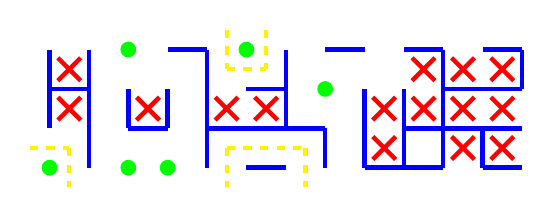
\begin{tikzpicture}[x=0.5cm, y=-0.5cm, ultra thick, blue]
% Walls
    \draw (3,0) -- (4,0);
    \draw (7,0) -- (8,0);
    \draw (9,0) -- (10,0);
    \draw (11,0) -- (12,0);
    \draw (0,1) -- (1,1);
    \draw (5,1) -- (6,1);
    \draw (10,1) -- (12,1);
    \draw (2,2) -- (3,2);
    \draw (4,2) -- (7,2);
    \draw (9,2) -- (12,2);
    \draw (5,3) -- (6,3);
    \draw (8,3) -- (10,3);
    \draw (11,3) -- (12,3);
    \draw (0,0) -- (0,2);
    \draw (1,0) -- (1,3);
    \draw (2,1) -- (2,2);
    \draw (3,1) -- (3,2);
    \draw (4,0) -- (4,3);
    \draw (6,0) -- (6,2);
    \draw (7,2) -- (7,3);
    \draw (8,1) -- (8,3);
    \draw (9,1) -- (9,3);
    \draw (10,0) -- (10,3);
    \draw (11,2) -- (11,3);
    \draw (12,0) -- (12,1);
% Pillars
    \fill[green] (2,0) circle(0.2);
    \fill[green] (5,0) circle(0.2);
    \fill[green] (7,1) circle(0.2);
    \fill[green] (0,3) circle(0.2);
    \fill[green] (2,3) circle(0.2);
    \fill[green] (3,3) circle(0.2);
% Inner points in accessible cul-de-sacs
    \node at (0.5,0.5) {};
    \node at (9.5,0.5) {};
    \node at (10.5,0.5) {};
    \node at (11.5,0.5) {};
    \node at (0.5,1.5) {};
    \node at (2.5,1.5) {};
    \node at (4.5,1.5) {};
    \node at (5.5,1.5) {};
    \node at (8.5,1.5) {};
    \node at (9.5,1.5) {};
    \node at (10.5,1.5) {};
    \node at (11.5,1.5) {};
    \node at (8.5,2.5) {};
    \node at (10.5,2.5) {};
    \node at (11.5,2.5) {};
% Entry-exit paths without intersections
    \draw[dashed, yellow] (4.5,0.5) -- (5.5,0.5);
    \draw[dashed, yellow] (-0.5,2.5) -- (0.5,2.5);
    \draw[dashed, yellow] (4.5,2.5) -- (6.5,2.5);
    \draw[dashed, yellow] (0.5,2.5) -- (0.5,3.5);
    \draw[dashed, yellow] (4.5,-0.5) -- (4.5,0.5);
    \draw[dashed, yellow] (4.5,2.5) -- (4.5,3.5);
    \draw[dashed, yellow] (5.5,-0.5) -- (5.5,0.5);
    \draw[dashed, yellow] (6.5,2.5) -- (6.5,3.5);
\end{tikzpicture}
\end{center}
\vspace*{\fill}

\end{document}
